\section{Real time systems}
% GOAL V01 • You can describe what an embedded real-time system is, how it can be built and what challenges may arise in such systems.

\subsection{Characteristics of embedded systems}
\begin{enumerate}
    \item \textbf{Interactivity}: They react via sensor input or actor output with the environment (event driven)
    \item \textbf{Efficient}: Resources are used effectively
    \item \textbf{Reliable, save}: They (should) always work predictively as designed
    \item \textbf{Specific}: They are specific for an application
    \item \textbf{Real time}: They achieve either hard or soft Real time requirements
    \item \textbf{External timing}: Typically the speed they operate on is dedicated from the outside
\end{enumerate}

\subsection{Real time systems definition}

\begin{minipage}{0.5\columnwidth}
Real time systems are computing system that \textbf{must} react within precise time constraints to events in the environment.
They are also characterized by a deadline.
Rather than being fast, a real time computing system is \textbf{predictable}.
Even in a worst case event where workload is the largest, they do not violate timing constraints.
Generally operating systems are used when multiple tasks have to be done simultaneously.
Core functions are:
\begin{itemize}
    \item Parallel processes and interprocess communication
    \item Abstract and provide driver for periphery
    \item Memory management, file systems
    \item General utilities (Clock, Math, Multi user)
\end{itemize}
\end{minipage}
\begin{minipage}{0.5\columnwidth}
    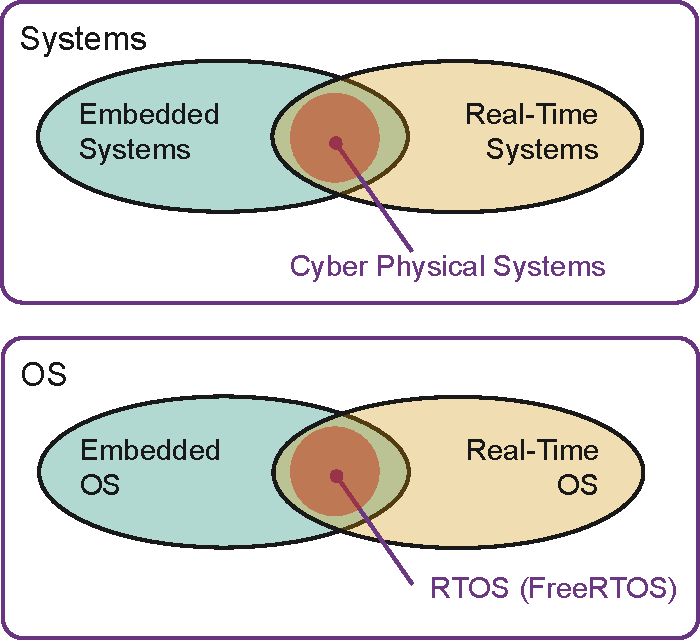
\includegraphics[width=\columnwidth]{images/PDF/System_OS.pdf}
\end{minipage}


% TODO v2
\subsection{RTOS vs. Bare-Metal}
% GOAL V02 • RTOS vs bare metal explanation

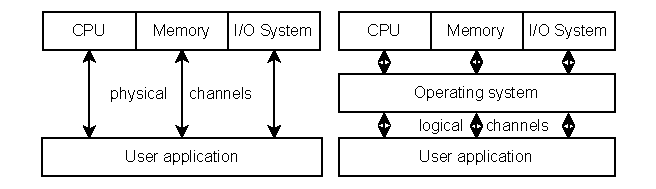
\includegraphics[width=\columnwidth]{images/PDF/Drawings-Bare-Metal vs. Embedded OS.pdf}

\begin{tabular}{clc}
    \textbf{User Program}                       & &\textbf{The operating system} \\\
    Directly, accesses real machine components  & & is a clear access abstraction \\
    Is closely coupled                          & & provides additional functionality\\
    uses a single super loop                    & & \\ 
\end{tabular}

\subsubsection{Advantages of staying bare metal}
\begin{itemize}
    \item Simple structure (for small applications)
    \item Low stack usage (only one stack required)
\end{itemize}

\subsubsection{Disadvantages of staying bare metal}
\begin{itemize}
    \item No “delay” capability
    \item Higher power consumption due to the lack of a power save mode in most architectures
    \item Difficult to maintain as program grows
    \item Timing of all software components depends on all other software components: Small change in one place can have major side effects in other places
    \item Defeats modular programming
    \item Real time behavior only with interrupts
\end{itemize}


\subsection{RTOS concepts and task management}
% GOAL V02 • tasks/processes, states, context switch, scheduling, multitasking, FreeRTOS

\subsubsection{Processes and tasks}
% (from V02 RTOS task management)

\subsubsection{Process states}

\subsubsection{Context switching}

\subsubsection{Scheduling and dispatching}

\subsubsection{Multitasking and concurrency}
% GOAL V02 • You can explain the principles of multitasking and concurrency.

\subsubsection{FreeRTOS task management}
% GOAL V02 • You can understand and utilize FreeRTOS to create and manage tasks.

\subsection{Components of a RTOS}

\begin{itemize}
    \item Scheduler
    \begin{itemize}
        \item Algorithm that determines when, which task is executed
        \item Allows for multitasking
    \end{itemize}
    \item Objects
    \begin{itemize}
        \item Kernel constructs that function as an API
        \item e.g. Tasks, semaphores, Message queues, \dots
    \end{itemize}
    \item Services
    \begin{itemize}
        \item Timing, interrupt handling, resources management like file systems
    \end{itemize}
\end{itemize}

\subsubsection{Execution modes and privilege levels}
Another important mechanism is the execution mode.
An OS has at least 2 privilege levels / modes for executing instructions.
The different modes are called \textbf{rings}.
Kernel mode (ring 0) allows for execution of all instructions.
User mode (ring 1,2,3,4) does \textbf{not allow} execution of all instructions


\subsection{Simple RTOS implementation}

\begin{center}
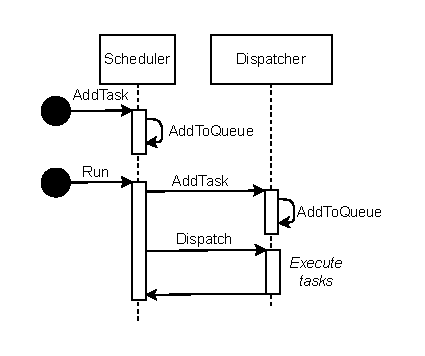
\includegraphics[width=0.6\columnwidth]{images/PDF/Scheduler.pdf}
\end{center}

When \verb|Addtaks| is called for a task, it is added to the queue.
The Scheduler periodically checks if tasks are ready.
If the task is ready to be called (Delay passed, sufficient priority), it is added to the dispatcher queue.
The scheduler calls the dispatcher queue, which executes all queued tasks.

\subsubsection{Scheduler}

\subsubsection{Dispatcher}

\begin{minipage}[t]{0.5\columnwidth}
    \lstinputlisting{code/Simple_Rtos_Dispatcher.hpp}
    \lstinputlisting{code/Simple_Rtos_Dispatcher.cpp}
\end{minipage}
\begin{minipage}[t]{0.5\columnwidth}
    \lstinputlisting{code/Simple_Rtos_Scheduler.hpp}
    The scheduler instantiates the dispatcher.
\end{minipage}

\lstinputlisting{code/Simple_Rtos_Scheduler.cpp}